% report.tex
% Scientific article template in English
% Recommended compilation: pdflatex report.tex -> biber report -> pdflatex report.tex (x2)

\documentclass[11pt,a4paper]{report}

% Encoding and language
\usepackage[T1]{fontenc}
\usepackage[utf8]{inputenc}
\usepackage[english]{babel}

% Page layout
\usepackage{geometry}
\geometry{margin=2.5cm}
\usepackage{microtype}
\usepackage{placeins}
% Graphics, tables, mathematics
\usepackage{graphicx}
\graphicspath{{../Images/}}
\usepackage{booktabs}
\usepackage{amsmath,amssymb,amsthm}
\usepackage{empheq}
\usepackage{siunitx}

% For floating algorithms with caption
\usepackage{algorithm}
%\usepackage{algorithmic}


\usepackage{algpseudocode}  % alternative to algorithmic, works with algorithm

% Links, citations
\usepackage[colorlinks=true,linkcolor=blue,citecolor=blue,urlcolor=blue]{hyperref}
\usepackage{csquotes}
% biblatex is loaded later with the desired options to avoid an "Option clash for package biblatex" error
\usepackage{minitoc}

% --------------------------------
% Reset chapter counter at each part
% --------------------------------
\makeatletter
\@addtoreset{chapter}{part}
\makeatother


\usepackage[
    backend=biber,
    style=numeric,   % <-- citations sous forme d'entiers
    sorting=none     % pour garder l'ordre d'apparition si tu veux
]{biblatex}

\addbibresource{../biblio.bib}

% Useful environments
\theoremstyle{plain}
\newtheorem{theorem}{Theorem}[section]
\theoremstyle{definition}
\newtheorem{definition}{Definition}[section]

% Handy commands
\newcommand{\ie}{\textit{i.e.}}
\newcommand{\eg}{\textit{e.g.}}

% PDF metadata
\hypersetup{
    pdftitle={Automated Calibration of Physical Models for Musical Instruments},
    pdfauthor={Rodolphe Milton VIVANT},
    pdffitwindow=true
}

\title{Automated Calibration of Physical Models for Musical Instruments\\[0.5em]}

\author{Rodolphe Milton VIVANT\thanks{UFR de Mathématique et Informatique de Strasbourg, rodolphe.vivant3@etu-unistra.fr}}
\date{\today}

\begin{document}
\dominitoc
\maketitle

\begin{abstract}
This project focuses on the automated calibration of physical models for reed musical instruments. 
We develop a numerical framework to simulate wave propagation inside instruments with variable cross-sectional areas using the Discontinuous Galerkin Method (DGM). 
Special attention is given to the implementation of boundary conditions that model radiation and reed dynamics. 
The framework is validated against analytical solutions for uniform cross-sections and extended to non-uniform geometries, such as exponential and conical profiles. 
Results demonstrate accurate wave propagation, proper handling of complex boundaries, and convergence consistent with theoretical expectations. 
The proposed approach provides a foundation for efficient parameter calibration in virtual instrument models.



\vspace{3em}
Ce projet porte sur la calibration automatique de modèles physiques pour les instruments de musique à anche. 
Nous développons un cadre numérique pour simuler la propagation des ondes à l'intérieur d'instruments présentant des sections transversales variables, en utilisant la méthode de Galerkin discontinu (DGM). 
Une attention particulière est portée à la mise en œuvre des conditions aux limites modélisant la radiation et la dynamique de l'anche. 
Le cadre est validé par rapport à des solutions analytiques pour des sections uniformes et étendu à des géométries non uniformes, telles que les profils exponentiels et coniques. 
Les résultats montrent une propagation des ondes précise, une gestion correcte des conditions aux limites complexes et une convergence conforme aux prédictions théoriques. 
Cette approche fournit une base solide pour la calibration efficace des paramètres dans les modèles d'instruments virtuels.
\end{abstract}

\newpage
\setcounter{tocdepth}{2}
\tableofcontents

\newpage
\chapter*{Introduction}
\addcontentsline{toc}{chapter}{Introduction}

During my project of the thrid semester of the CSMI Master degree, I worked on the automated calibration 
of physical models for musical instruments. 
The goal of this project was to develop a method to automatically adjust the parameters of physical models 
so that they accurately reproduce the characteristic sounds of reed instruments. \newline
I worked under the supervision of Dr Emmanuel Franck, Dr Laurent Navoret and Dr Victor Michel-Dansac from 
the Institut de Recherche Mathématique Avancée (IRMA) in Strasbourg and Dr Juliette Chabassier from Modartt. \newline
Modartt (MOdels and Data for ARTs and Technology)\cite{Modartt} is a french company specialized in the development of artistic and technological application softwares.
In 2006, they released \textit{Pianoteq}, a software that simulates the sound of various musical instruments using physical modeling techniques isntead 
of relying on pre-recorded samples. \newline
First, we present the context of reed instruments and the state of the art of the mathematical modeling of the wave equation inside these instruments.
Then, we describe the numerical methods used to solve the wave equation with different types of cross-sectional 
area (uniform, exponential, conical) using the Discontinuous Galerkin Method (DGM). We will particularly focus on the implementation of the boundary conditions
that represent a crucial aspect of the behavior of the sound produced by the instrument.
Finally, we present the results of the numerical simulations and the performance analysis of the implemented method.


\newpage
\section*{Reed Instruments}
A reed is a thin, flexible lamina mounted at the mouthpiece or at the entrance of an air column resonator that acts \cite{Universalis_Anche} \cite{chaigne:hal-05370840} as a valve that controls the airflow driven by a pressure difference between the upstream region 
(the player’s mouth) and the downstream region (the mouthpiece or mouthpiece tip of the instrument). \newline
There are two principal categories of reed instruments:
\begin{itemize}
    \item Free reeds (harmonicas, accordions, ...).
    \item Beating reeds (clarinets, saxophones, ...).
\end{itemize}
% Figure : schéma de l'anche / embouchure
\begin{figure}[htbp]
    \centering
    % Remplacez 'figs/reed.png' par le chemin et l'extension réels de votre image (pdf, png, jpg...)
    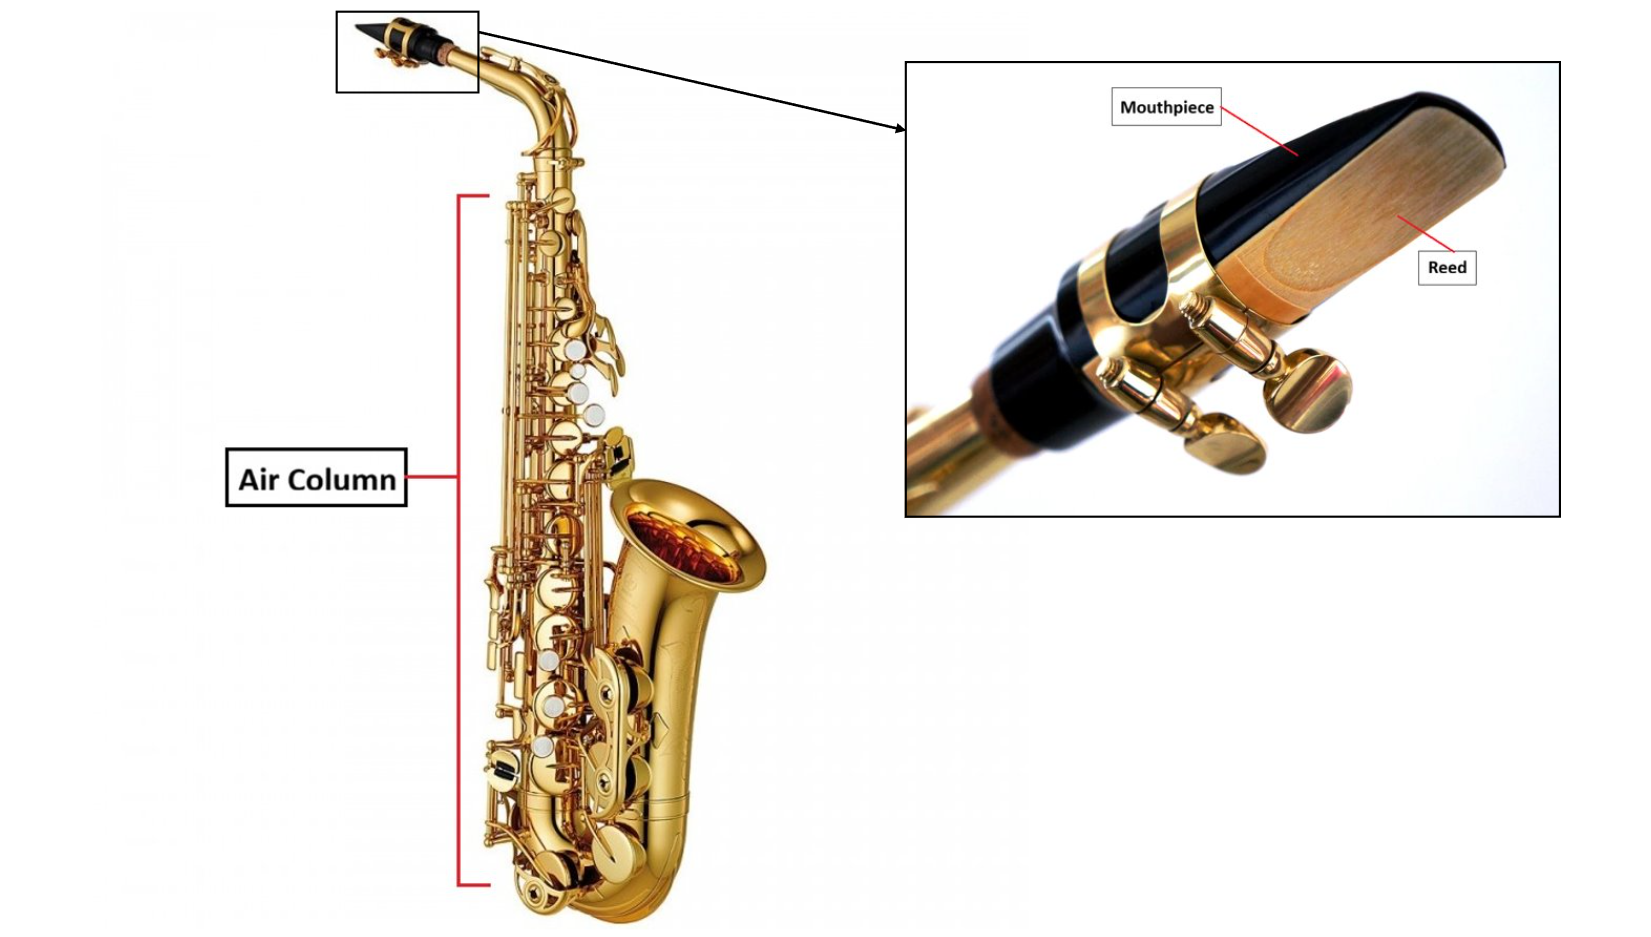
\includegraphics[width=0.75\textwidth]{reed_column.png}
    \caption{Reed and saxophone.}
    \label{fig:reed_schematic}
\end{figure}

\section*{Objectives}
The main objectives of this project are: \\
In JAX framework:
\begin{enumerate}
    \item Implement a discontinous Galerkin discretization of the mixed form of the wave equation and numerically solve it.
    \item Implement the Left Hand Side boundary conditions (equations \eqref{eq:1c} and \eqref{eq:1d}) coupled with the DG solver.
    \item Implement the Right Hand Side boundary conditions (equations \eqref{eq:1e} and \eqref{eq:1f}) coupled with the DG solver.
    \item Compute the gradient with respect to all the problem parameters.   
\end{enumerate}

\part{Direct Resolution}

\chapter{Physical Model}

The equations governing the behavior of reed instruments are mathematically described \cite{MAMAMIA2024} by a set of coupled 
differential equations (Partial Differential Equations - PDEs, Ordinary Differential Equations - ODEs, and 
algebraic equations). These equations capture the complex interactions between the pressure ($p$), the acoustic
volume velocity ($v$) \eqref{eq:1a} \eqref{eq:1b}, radiative phenomenons happening at the bell of the instrument($\phi$) \eqref{eq:1c} \eqref{eq:1d}, 
and the effects of the instrumental player \eqref{eq:1e} \eqref{eq:1f} :

% Système d'équations décrivant un modèle réducteur pour un instrument à anche
\begin{subequations}
\begin{empheq}[left=\empheqlbrace]{align}
\frac{S(x)}{c S^\ast}\,\partial_t p(x,t) + \partial_x v(x,t) &= 0 \label{eq:1a}\\[4pt]
\frac{S^\ast}{c S(x)}\,\partial_t v(x,t) + \partial_x p(x,t) &= 0 \label{eq:1b}\\[4pt]
Z^\ast_T\,\partial_t \phi + \sqrt{\alpha}\,p(L,t) &= 0 \label{eq:1c}\\[4pt]
-\frac{\beta}{Z^\ast_T}\,p(L,t) + v(L,t) + \sqrt{\alpha}\,\phi &= 0 \label{eq:1d}\\[4pt]
-v(0,t) + \zeta \ell(y)\,F(\gamma - p(0,t)) + \varepsilon\frac{\kappa}{\omega_r}\,\partial_t y &= 0 \label{eq:1e}\\[6pt]
\frac{1}{\omega_r^2}\,\partial_{tt} y + \frac{1}{Q_r\omega_r}\,\partial_t y + y - 1 
&= \varepsilon(\gamma - p(0,t)) \label{eq:1f}
\end{empheq}
\end{subequations}

where $S(x)$ is the cross-sectional area of the instrument at position $x$, $S^\ast$ is a reference area,
$c$ is the speed of sound, $Z^\ast_T$ is a reference acoustic impedance, 
$\alpha$ and $\beta$ are parameters related to the radiation effects, $L$ is the length of the instrument,
$\zeta_\ell(y)$ is a function representing the lip-reed coupling, $F$ is a nonlinear function ($F(\Delta p)=\Delta p \, \text{sign} (\Delta p)$),
$\gamma$ is the dimensionless blowing pressure, $\varepsilon$ =-1 for a reed instrument, 
$\kappa$ is a parameter related to the lip dynamics, $\omega_r$ is the reed's (or lips') frequency ($=2\pi f_r$), 
$Q_r$ is the quality factor of the reed, and $y$ is the dimensionless reed opening. \newline
This kind of system of equation can already be solved numerically with Openwind \cite{OpenwindInria}.

\minitoc

\section{Conservative formulation}
The main issue with the latter formulation is that the first two equations \eqref{eq:1a} and \eqref{eq:1b} are not in conservative form, 
which makes it difficult to apply the Discontinuous Galerkin Method (DGM) for numerical resolution.
To address this issue, we introduce the following change of variables:
\begin{equation}
\tilde{u} = 
\begin{pmatrix}
    \tilde{p} \\ \tilde{v}
\end{pmatrix} 
= 
\begin{pmatrix}
    \frac{S(x)}{c S^\ast}\,p \\ \frac{S^\ast}{c S(x)}\,v
\end{pmatrix}
\end{equation}

The system of equations can then be rewritten in a conservative form as follows:
\begin{equation}
    \partial_t \tilde{u} + \partial_x F(\tilde{u}) = \partial_t \tilde{u} + \partial_x (A(x)\tilde{u}) = 0
\end{equation}
where $A(x) = \begin{pmatrix}
    0 & \frac{c S(x)}{S^\ast} \\ \frac{c S^\ast}{S(x)} & 0
\end{pmatrix}$ is the flux matrix. 
\newline

From this change of variables, we can also compute the Riemann invariants of the system, which are given by:
(démo)
\begin{equation}
    w^\pm = \tilde{v} \pm \kappa\tilde{p}
\end{equation}
where $\kappa = \left(\frac{S(x)}{cS^\ast}\right)^2$. \newline
These Riemann invariants represent the characteristic variables of the system 
They appear to be very useful for understanding the wave propagation and for implementing boundary conditions.

\section{Radiation Boundary Conditions}

The right boundary condition at $x=L$ is modeled by the coupled system
\begin{equation}
\begin{cases}
Z^\ast_T\,\partial_t \phi(t)
+ \sqrt{\alpha}\, p(L,t) = 0,
\\[0.4em]
-\dfrac{\beta}{Z^\ast_T}\, p(L,t)
+ v(L,t)
+ \sqrt{\alpha}\,\phi(t) = 0.
\end{cases}
\label{eq:bc_ode_pde}
\end{equation}

The first equation governs the temporal evolution of the boundary variable
$\phi(t)$, while the second equation defines a dynamic impedance relation
between pressure and velocity at the boundary. Rewriting the second equation yields
\begin{equation}
v(L,t)
=
\frac{\beta}{Z^\ast_T} p(L,t)
-
\sqrt{\alpha}\,\phi(t).
\tag{BC}
\end{equation}

Introducing the transformed variables
\[
\tilde p
=
\frac{S(x)}{cS^\ast}p,
\qquad
\tilde v
=
\frac{S^\ast}{cS(x)}v,
\]
the boundary condition becomes
\begin{equation}
\frac{cS_L}{S^\ast}\tilde v(L,t)
=
\frac{\beta}{Z^\ast_T}
\frac{cS^\ast}{S_L}\tilde p(L,t)
-
\sqrt{\alpha}\,\phi(t),
\end{equation}
where $S_L = S(L)$.

Dividing by $\dfrac{cS_L}{S^\ast}$ gives
\begin{equation}
\tilde v(L,t)
=
\frac{\beta}{Z^\ast_T}
\left(
\frac{S^\ast}{S_L}
\right)^2
\tilde p(L,t)
-
\frac{S^\ast}{cS_L}
\sqrt{\alpha}\,\phi(t).
\end{equation}

We now introduce the characteristic variables
\begin{equation}
w^\pm
=
\tilde v
\pm
\kappa \tilde p,
\qquad
\kappa
=
\left(
\frac{S_L}{cS^\ast}
\right)^2.
\end{equation}

Hence,
\begin{equation}
\tilde v
=
\frac{w^+ + w^-}{2},
\qquad
\tilde p
=
\frac{w^+ - w^-}{2\kappa}.
\end{equation}

Substituting these expressions into the boundary condition yields
\begin{equation}
\frac{w^+ + w^-}{2}
=
\frac{\beta}{Z^\ast_T}
\left(
\frac{S^\ast}{S_L}
\right)^2
\frac{w^+ - w^-}{2\kappa}
-
\frac{S^\ast}{cS_L}
\sqrt{\alpha}\,\phi(t).
\end{equation}

Defining
\[
A
=
\frac{\beta}{Z^\ast_T}
\left(
\frac{S^\ast}{S_L}
\right)^2,
\qquad
B
=
\frac{S^\ast}{cS_L}\sqrt{\alpha},
\]
we obtain
\begin{equation}
w^-
\left(
1+\frac{A}{\kappa}
\right)
=
w^+
\left(
\frac{A}{\kappa}-1
\right)
-
2B\phi(t),
\end{equation}
and therefore
\begin{equation}
w^-
=
\frac{\dfrac{A}{\kappa}-1}
     {1+\dfrac{A}{\kappa}}
\, w^+
-
\frac{2B}
     {1+\dfrac{A}{\kappa}}
\, \phi(t).
\end{equation}

This relation provides the incoming characteristic variable $w^-$
as a function of the outgoing characteristic $w^+$ and the boundary
state variable $\phi(t)$.

\section{Reed Model}
The left-hand side boundary conditions \eqref{eq:1e} and \eqref{eq:1f} represent the coupling between the acoustic field inside the instrument and the dynamics of the reed.



\chapter{Numerical Methods}
\minitoc
\section{Discontinuous Galerkin Formulation}
\section{Numerical Fluxes}
\section{Time Integration}

\chapter{Numerical Results}
\minitoc
\section{Validation}
\subsection{Case $S(x)=const$}
\subsubsection{Analytical vs numerical solution}
\subsubsection{Convergence analysis}
\subsection{Case $S(x)$ variates}
\section{Reed Oscillations}
\subsection{Performances}

\chapter{Conclusion}

\part{Automated Calibration}

\chapter{Calibration Strategy}
\minitoc

\chapter{Spectral Losses}
\minitoc
\section{STFT}
\section{Spectrograms}
\subsection{}

\chapter{Neural Architectures}
\minitoc

\chapter{Perspectives}
\minitoc

\part*{General Conclusion}
\addcontentsline{toc}{part}{Conclusion}

\newpage
\part*{Appendix}
\addcontentsline{toc}{part}{Appendix}
\section*{Use of Artificial Intelligence Assistance}

Some parts of this work were prepared with the assistance of Artificial Intelligence (AI) tools.  
The following tools were used, with all outputs systematically verified, revised, and responsibly integrated by the authors:

\begin{itemize}
    \item \textbf{ChatGPT} (OpenAI, GPT-4 / GPT-5 family) – used to support code development, documentation, and methodological clarification, as well as to assemble an introductory bibliography.
\end{itemize}

The AI assistance was limited to the following explicit prompts:

\begin{itemize}
    \item \textit{Create a function to read arguments from the execution command}
    \item \textit{How to create an organigram of my repository in a Markdown file}
    \item \textit{How to fill a \texttt{.bib} file}
    \item \textit{Why my ghost cells are not being properly taken into account}
    \item \textit{Create a Python script to convert CSV $\rightarrow$ \LaTeX{} $\rightarrow$ PDF}
    \item \textit{Give examples of cross-section functions for reed instruments}
    \item \textit{Give an example of a compactly supported function}
    \item \textit{Improve the formulation of the following algorithm}
    \item \textit{How to include a sub-table of contents in each section}
    \item \textit{Improve the commentaries on the following code snippet}
\end{itemize}

All AI-generated outputs were carefully verified, adapted, and corrected by the authors.  
The authors take full responsibility for the accuracy, originality, and scientific integrity of this work.

\newpage
\printbibliography

% Minimal example of an external bibliography (create refs.bib)
% Example BibTeX entry:
%
% @article{doe2020,
%   author = {Doe, John and Example, Anne},
%   title = {Title of the cited article},
%   journal = {Example Journal},
%   year = {2020},
%   volume = {12},
%   pages = {34--56}
% }

\end{document}